\documentclass[a4paper,10pt,openany]{article}
\usepackage{fancyhdr}
\usepackage[T1]{fontenc}
\usepackage[margin=1.8cm]{geometry}
\usepackage[applemac]{inputenc}
\usepackage{lmodern}
\usepackage{enumitem}
\usepackage{microtype}
\usepackage{hyperref}
\usepackage{enumitem}
\usepackage{dsfont}
\usepackage{amsmath,amssymb,amsthm}
\usepackage{mathenv}
\usepackage{amsthm}
\usepackage{graphicx}
\usepackage[all]{xy}
\usepackage{lipsum}       % for sample text
\usepackage{changepage}
\theoremstyle{plain}
\newtheorem{thm}{Theorem}[section]
\newtheorem*{thm*}{Th\'eor\`eme}
\newtheorem{prop}[thm]{Proposition}
\newtheorem{cor}[thm]{Corollary}
\newtheorem{lem}[thm]{Lemma}
\newtheorem{propr}[thm]{Propri\'et\'e}
\theoremstyle{definition}
\newtheorem{deff}[thm]{Definition}
\newtheorem{rqq}[thm]{Remark}
\newtheorem{ex}[thm]{Exercice}
\newcommand{\e}{\mathrm{e}}
\newcommand{\prodscal}[2]{\left\langle#1,#2\right\rangle}
\newcommand{\devp}[3]{\frac{\partial^{#1} #2}{\partial {#3}^{#1}}}
\newcommand{\w}{\omega}
\newcommand{\dd}{\mathrm{d}}
\newcommand{\x}{\times}
\newcommand{\ra}{\rightarrow}
\newcommand{\pa}{\partial}
\newcommand{\vol}{\operatorname{vol}}
\newcommand{\dive}{\operatorname{div}}
\newcommand{\T}{\mathbf{T}}
\newcommand{\R}{\mathbf{R}}
\newcommand{\Q}{\mathbf{Q}}
\newcommand{\Z}{\mathbf{Z}}
\newcommand{\N}{\mathbf{N}}
\newcommand{\C}{\mathbf{C}}
\newcommand{\F}{\mathcal{F}}
\newcommand{\Homeo}{\mathrm{Homeo}}
\renewcommand{\x}{\mathbf{x}}
\newcommand{\Matn}{\mathrm{Mat}_{n \times n}}
\DeclareMathOperator{\tr}{tr}
\newcommand{\id}{\mathrm{id}}
\newcommand{\htop}{h_\mathrm{top}}


\title{\textsc{Syst\`emes dynamiques} \\ Feuille d'exercices 9}
\date{}
\author{}

\begin{document}

{\noindent \'Ecole Normale Sup\'erieure  \hfill \texttt{chaubet@dma.ens.fr} } \\
{2020/2021 \hfill }

{\let\newpage\relax\maketitle}
\maketitle

\noindent {\large \textbf{Exercice 1.} \textit{Exemples de mesures invariantes}} \vspace{1.5mm} 

\noindent Montrer que la mesure $\mu$ est conserv\'ee par la transformation $f : X \to X$ (d\'efinie $\mu$-pp) dans les cas suivants.
\begin{enumerate}
\item $X = [0,1]$, $\dd \mu(x) = \displaystyle{\frac{\dd x}{2\sqrt{1-x}}}$ et $f(x) = 2 \sqrt{x(1-x)}$.
\item $X$ est une vari\'et\'e, $f : X \to X$ est un diff\'eomorphisme, $x$ est un point p\'eriodique de p\'eriode $n$ pour $f$ et $\displaystyle{
\mu = \frac{1}{n} \sum_{k=1}^n \delta_{f^k(x)}.
}
$
\item $X = [0,1]$, $\mu$ est la mesure de Lebesgue et
$ \displaystyle{
f(x) = \left\{ \begin{matrix} 2x \quad &\text{ si }\quad  0\leq x \leq 1/2, \\ 2 -2x \quad &\text{ si } \quad 1/2 < x \leq 1. \end{matrix}\right.
}
$
\item $X = \R^d/\Z^d$ est le tore de dimension $d$, $\mu$ est la mesure de Haar sur $X$ et $f$ est un automorphisme de $X$.
\item $X = [0,1]$, $\dd \mu(x) = \displaystyle{\frac{\dd x}{\log2(1+x)}}$ et $\displaystyle{f(x) = \frac{1}{x} - \left[\frac{1}{x}\right]}$, o\`u $[y]$ est la partie enti\`ere d'un r\'eel $y$.
\end{enumerate}

\vspace{0.6cm}

\noindent {\large \textbf{Exercice 2.} \textit{Version topologique du th\'eor\`eme de r\'ecurrence de Poincar\'e}} \vspace{1.5mm} 

\noindent Soit $M$ un espace topologique \`a base d\'enombrable et $f : M \to M$ une transformation continue. On dira que $x \in M$ est r\'ecurrent pouf $f$ si pour tout voisinage $U$ de $x$, il existe $n>0$ tel que $f^n(x) \in U$. Soit $\mu$ une mesure bor\'elienne finie sur $M$ invariante par $f$. Montrer que $\mu$-presque tout point de $M$ est r\'ecurrent pouf $f$. 
\vspace{0.6cm}

\noindent {\large \textbf{Exercice 3.} \textit{Existence de mesures invariantes}} \vspace{1.5mm} 

\noindent Soit $(X, \dd)$ un espace m\'etrique compact. On note $E = \mathcal{C}(X,\C)$ l'espace de Banach des fonctions continues sur $X$ muni de la norme
$$
\| f \| = \sup_{X} |f|,
$$
et $E^*$ l'espace des formes lin\'eaires continues sur $E$, muni de la norme 
$$
\|L\|_* = \sup_{\| f \| \leq 1} |L(f)|. 
$$
On dira qu'une suite $(L_n)$ de $E^*$ converge $*$-faiblement vers $L \in E^*$ si pour tout $f \in E$ on a $L_n(f) \to L(f)$.
\begin{enumerate}
\item Soit $(f_i) \subset E$ une suite dense dans $E$. On note $\displaystyle{\dd_*(L,L') = \sum_{i=0}^\infty \frac{|L(f_i)-L'(f_i)|}{2^i (1+\|f_i\|)}}$. Montrer que $\dd_*$ est une distance sur la boule unit\'e de $E^*$ et que la topologie engendr\'ee co\"incide avec la topologie $*$-faible.
\item En d\'eduire que la boule unit\'e de $E^*$ est compacte pour la topologie $*$-faible.
\item Soit $f : X \to X$ une transformation continue. Montrer que l'ensemble des mesures de probabilit\'es sur $X$ invariantes par $f$ est non vide, connexe, et ferm\'e dans l'ensemble des mesures de probabilit\'es sur $X$ (pour la topologie faible-$*$).
\end{enumerate}
\vspace{0.6cm}

\noindent {\large \textbf{Exercice 4.} \textit{Fonctions harmoniques sur une vari\'et\'e ferm\'ee}} \vspace{1.5mm} 

\noindent Soit $M$ une vari\'et\'e connexe compacte sans bord, et $g$ une m\'etrique sur $M$, c'est-\`a-dire la donn\'ee d'un produit scalaire $g_x$ sur $T_xM$ en tout point $x\in M$ et d\'ependant de mani\`ere lisse de $x$. La mesure de volume $\vol_g$ est donn\'ee en cordonn\'ees $(x^1, \dots, x^n)$ par 
$$
\sqrt{|g|}~ \dd x^1 \cdots \dd x^n,
$$
o\`u $|g|(x) = \displaystyle{\det\bigl(g_{ij}(x)\bigr)}$ ; ici $(g_{ij}(x))$ est la matrice repr\'esentant $g$ au point $x$ dans la base $\partial_1, \dots, \partial_n$, o\`u $\partial_j = \displaystyle{\frac{\partial}{\partial x^j}}$. Si $X$ est un champ de vecteurs sur $M$, on d\'efinit sa divergence $\mathrm{div}_g X \in \mathcal{C}^\infty(M)$ localement par
$$
\mathrm{div}_g(X) = \frac{1}{\sqrt{|g|}}\sum_{j=1}^n \partial_j \left(\sqrt{|g|}X^j\right), \quad X = \sum_{j=1}^n X^j \partial_j.
$$
On admet que ces d\'efinitions ne d\'ependent pas du syst\`eme de coordonn\'ees choisi.
\begin{enumerate}
\item Montrer que le flot de $X$ pr\'eserve $\vol_g$ si et seulement si $\mathrm{div}_g(X) = 0$.
\end{enumerate}
Pour $\varphi \in \mathcal{C}^\infty(M)$, on note $\nabla^g \varphi$ le gradient le $\varphi$, c'est-\`a-dire le champ de vecteurs sur $M$ d\'efini par 
$$
\dd_x \varphi \cdot v = g(\nabla^g \varphi (x),v), \quad x \in M, \quad v \in T_xM.
$$
On d\'efinit aussi l'op\'erateur de Laplace-Beltrami $\Delta_g = \mathrm{div}_g \nabla^g$ et on dira que $\varphi \in \mathcal{C}^\infty(M)$ est harmonique si $\Delta_g \varphi = 0$.
\begin{enumerate}[resume]
\item Montrer que toute fonction harmonique sur $M$ est constante.
\end{enumerate}
\vspace{0.6cm}


\noindent {\large \textbf{Exercice 5.} \textit{Transformation du billard}} \vspace{1.5mm} 

\noindent On consid\`ere le cercle $S^1 = \bigl\{(x,y) \in \R^2, ~x^2 + y^2 = 1\bigr\} \subset \R^2$, et on note $M = S^1 \times \left]-\pi/2, \pi/2\right[$. On consid\`ere une particule qui se d\'eplace dans le disque \`a vitesse constante et qui rebondit de mani\`ere parfaite sur le bord. Un \'etat initial $(q_0, \theta_0) \in M$ d\'etermine enti\`erement les rebonds $(q_n, \theta_n) \in M$ pour $n \in \N$ (cf. Figure \ref{fig:1}).


\begin{enumerate}
\item Exprimer $(q_n, \theta_n)$ en fonction de $(q_0, \theta_0)$. Montrer que la trajectoire $(q_n, \theta_n)$ est p\'eriodique si et seulement si $\theta_0 \in \pi \Q$. Calculer le nombre $t$ de tours et le nombre $r$ de rebonds effectu\'es en fonction de $p,q \in \Z$ premiers entre eux o\`u $\theta_0 = \pi p / q.$
%\item On suppose $\theta_0 = \pi \alpha$ avec $\alpha \in \R \setminus \Q$ et soit $I$ un intervalle de $S^1$. Montrer que 
%$$
%\frac{1}{n}\# \bigl\{k \in \{0, \dots, n-1\}, ~q_k \in I \bigr\} \underset{n \to \infty}{\longrightarrow} \frac{|I|}{2\pi},
%$$
%o\`u $|I|$ est la longueur de $I$.
\item Montrer que la transformation $T : M \to M$ d\'efinie par $T(q_0, \theta_0) = (q_1, \theta_1)$ pr\'eserve la mesure $\ell \otimes (\cos \theta~ \dd \theta)$ sur $M$, o\`u $\ell$ est la mesure de Lebesgue sur $S^1$.
\end{enumerate}
On consid\`ere maintenant une courbe lisse simple (pas d'autointersection) $\gamma : S^1 \to \R^2$ param\'etr\'ee par longueur d'arc et d\'elimitant un ouvert $\Omega$ strictement convexe et born\'e, et on consid\`ere $M_\gamma = \gamma(S^1) \times \left]-\pi/2, \pi/2 \right[$. On consid\`ere la dynamique de billard $T_\gamma : M_\gamma \to M_\gamma$ comme dans le cas du cercle (cf. Figure \ref{fig:1}).

\begin{enumerate}[resume]
\item Montrer que $T_\gamma$ pr\'eserve la mesure $\gamma_* \ell \otimes (\cos \theta ~\dd \theta)$.
\end{enumerate}

\begin{figure}[h!]
\begin{center}
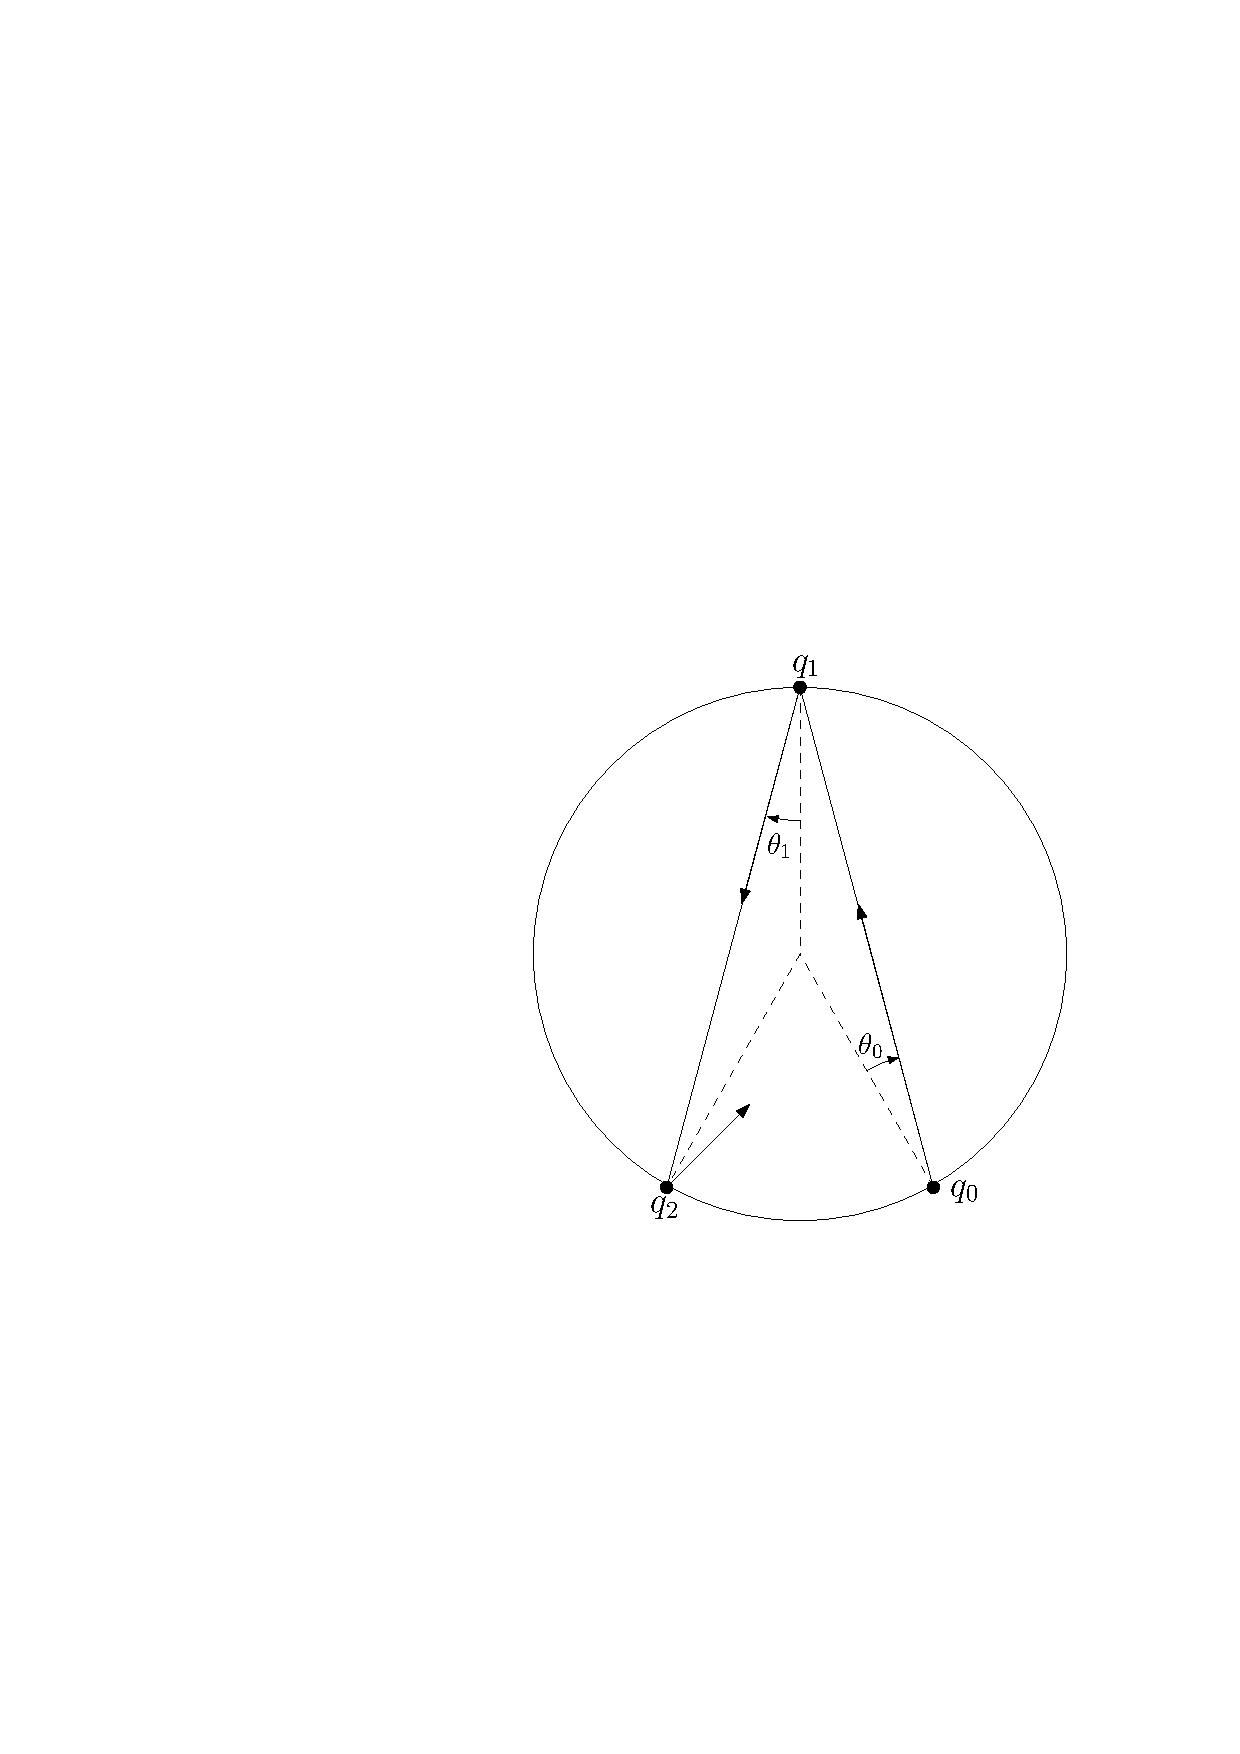
\includegraphics[width=5cm]{billard.pdf}
\hspace{2cm}
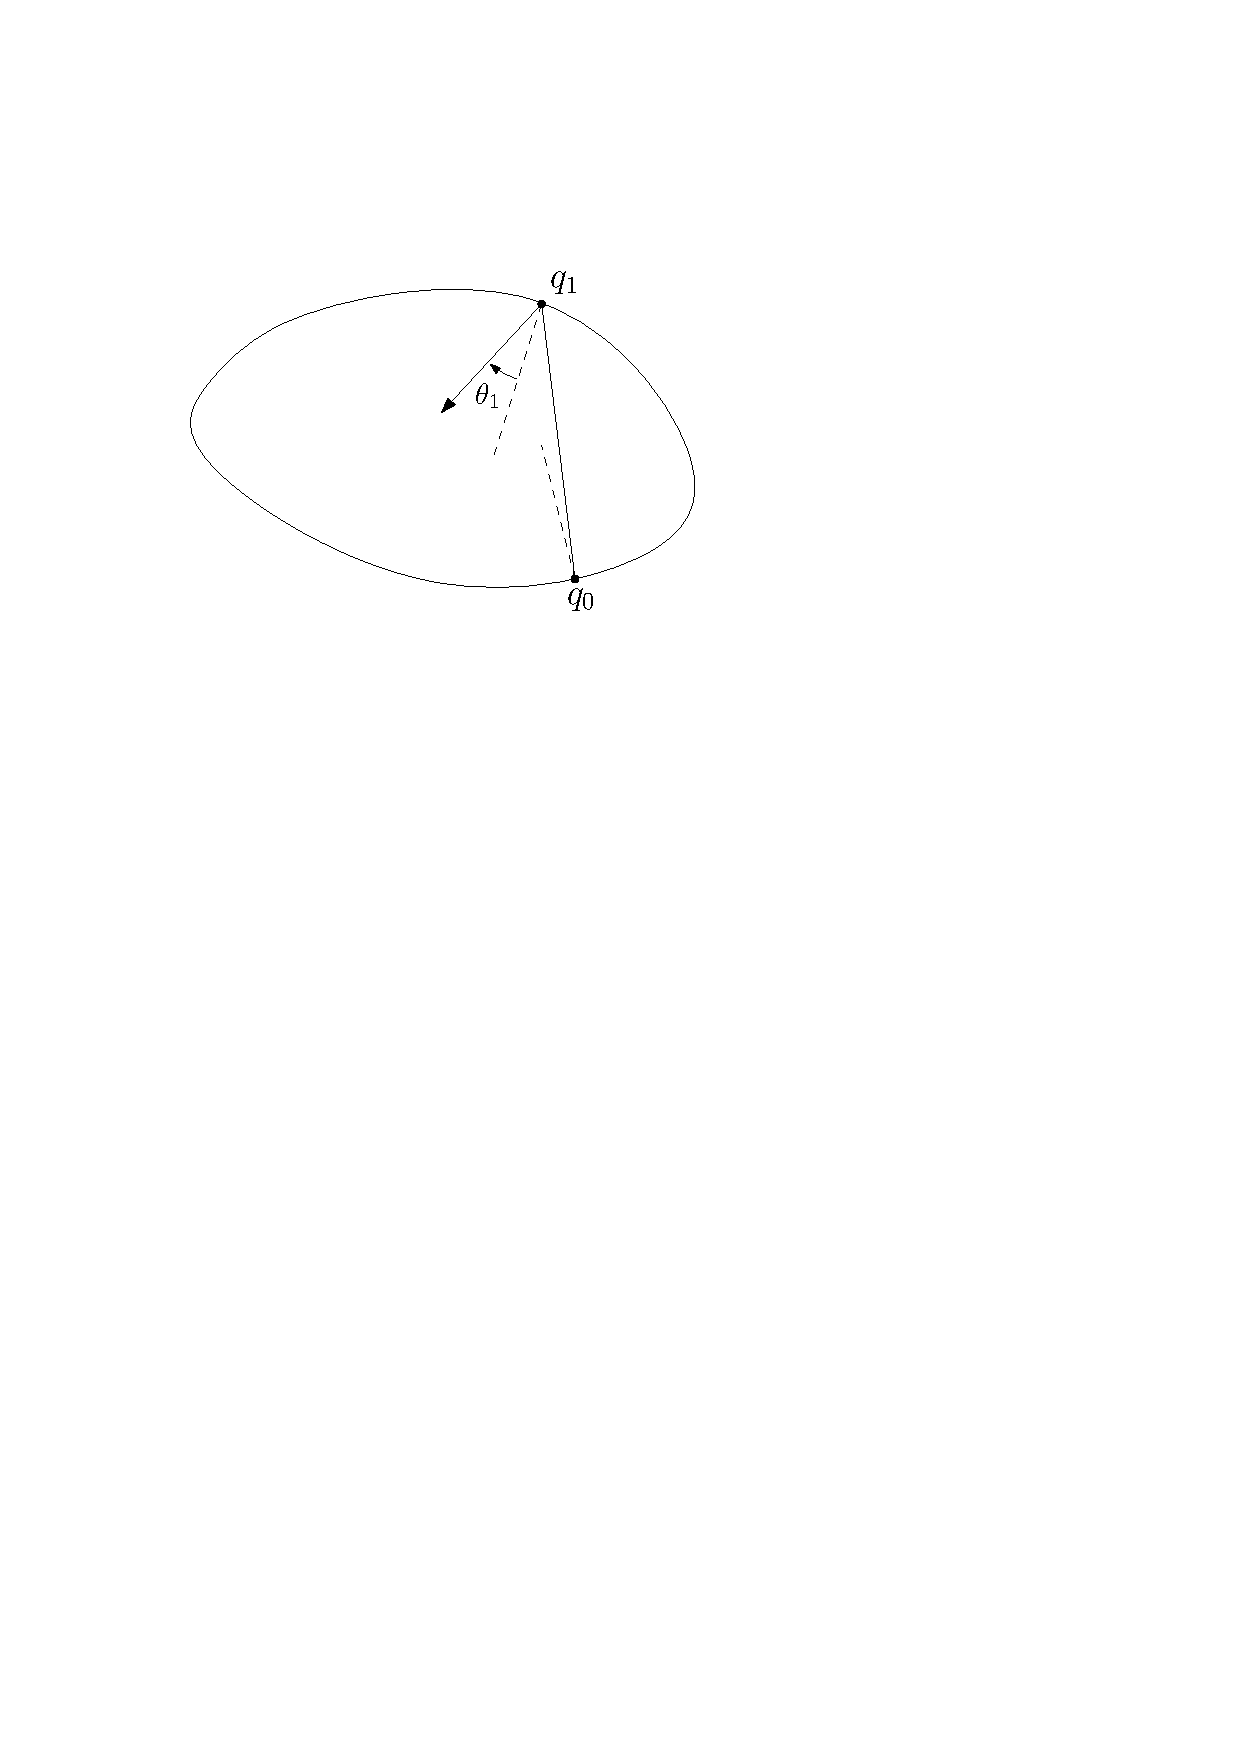
\includegraphics[width=5cm]{billard2.pdf}
\end{center}
\caption{\'Evolution d'une particule dans un billard}
\label{fig:1}
\end{figure}

\noindent {\large \textbf{Exercice 6.} \textit{Application de retour d'une rotation sur le cercle}} \vspace{1.5mm} 

\noindent Soit $I = [a,b] \subset [0,1]$ un intervalle. On dit qu'une transformation $T : I \to I$ est un \'echange de trois intervalles s'il existe $a\leq c \leq d \leq b$ tels que
$$T\bigl([a,c)\bigr) = [d,b), \quad T\bigl([c,d)\bigr) = [c,d), \quad T\bigl([d,b)\bigr) = [a,c),$$
et tels que $T$ est affine et croissante sur chacun des intervalles pr\'ec\'edents. Montrer que l'application de retour sur un intervalle associ\'ee \`a une rotation du cercle est un \'echange de trois intervalles.




\end{document}

\noindent {\large \textbf{Exercice 8.} \textit{Flots hamiltoniens}} \vspace{1.5mm} 

\noindent Soit $H : \R^{2n} \to \R$ une fonction lisse. Le champ hamiltonien $X$ associ\'e \`a $H$ est le champ de vecteurs sur $\R^{2n}$ d\'efini par

$$ X(x, \xi) = J \cdot \nabla H (x,\xi), \quad (x,\xi) \in \R^{2n},$$
o\`u $J = \begin{pmatrix} 0 & I_n \\ -I_n & 0 \end{pmatrix}$. On suppose qu'il existe une application lisse $A : \R^n \to S_n(\R)$ telle que $A(x)$ est d\'efinie positive pour tout $x$ et
$$
H(x,\xi) = \frac{1}{2} \bigl\langle A(x)\xi, \xi \bigr\rangle, \quad (x,\xi) \in \R^{2n}.
$$
\vspace{0.6cm}




\end{document}
 
